% Created by tikzDevice version 0.12.3 on 2020-08-02 16:17:51
% !TEX encoding = UTF-8 Unicode
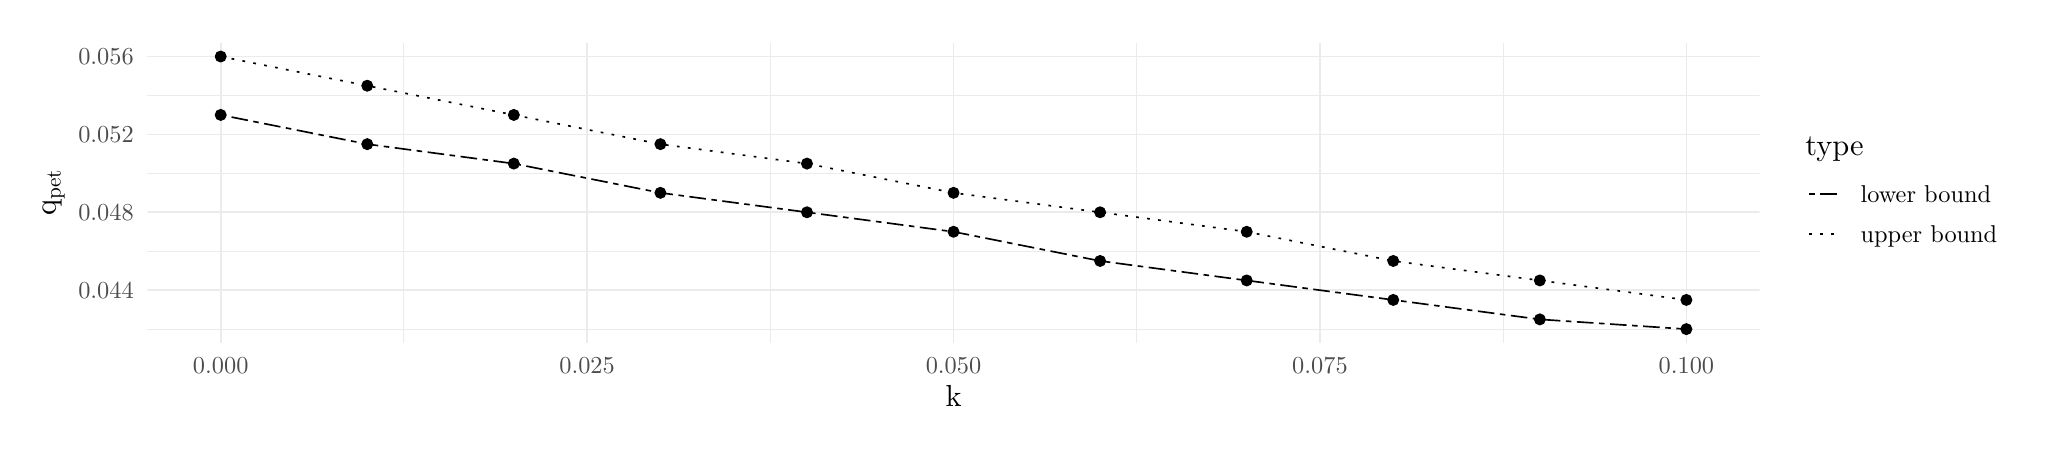
\begin{tikzpicture}[x=1pt,y=1pt]
\definecolor{fillColor}{RGB}{255,255,255}
\path[use as bounding box,fill=fillColor,fill opacity=0.00] (0,0) rectangle (722.70,144.54);
\begin{scope}
\path[clip] ( 43.27, 30.69) rectangle (625.86,139.04);
\definecolor{drawColor}{gray}{0.92}

\path[draw=drawColor,line width= 0.3pt,line join=round] ( 43.27, 35.61) --
	(625.86, 35.61);

\path[draw=drawColor,line width= 0.3pt,line join=round] ( 43.27, 63.75) --
	(625.86, 63.75);

\path[draw=drawColor,line width= 0.3pt,line join=round] ( 43.27, 91.90) --
	(625.86, 91.90);

\path[draw=drawColor,line width= 0.3pt,line join=round] ( 43.27,120.04) --
	(625.86,120.04);

\path[draw=drawColor,line width= 0.3pt,line join=round] (135.95, 30.69) --
	(135.95,139.04);

\path[draw=drawColor,line width= 0.3pt,line join=round] (268.36, 30.69) --
	(268.36,139.04);

\path[draw=drawColor,line width= 0.3pt,line join=round] (400.76, 30.69) --
	(400.76,139.04);

\path[draw=drawColor,line width= 0.3pt,line join=round] (533.17, 30.69) --
	(533.17,139.04);

\path[draw=drawColor,line width= 0.6pt,line join=round] ( 43.27, 49.68) --
	(625.86, 49.68);

\path[draw=drawColor,line width= 0.6pt,line join=round] ( 43.27, 77.83) --
	(625.86, 77.83);

\path[draw=drawColor,line width= 0.6pt,line join=round] ( 43.27,105.97) --
	(625.86,105.97);

\path[draw=drawColor,line width= 0.6pt,line join=round] ( 43.27,134.11) --
	(625.86,134.11);

\path[draw=drawColor,line width= 0.6pt,line join=round] ( 69.75, 30.69) --
	( 69.75,139.04);

\path[draw=drawColor,line width= 0.6pt,line join=round] (202.15, 30.69) --
	(202.15,139.04);

\path[draw=drawColor,line width= 0.6pt,line join=round] (334.56, 30.69) --
	(334.56,139.04);

\path[draw=drawColor,line width= 0.6pt,line join=round] (466.97, 30.69) --
	(466.97,139.04);

\path[draw=drawColor,line width= 0.6pt,line join=round] (599.37, 30.69) --
	(599.37,139.04);
\definecolor{drawColor}{RGB}{0,0,0}

\path[draw=drawColor,line width= 0.6pt,dash pattern=on 2pt off 2pt on 6pt off 2pt ,line join=round] ( 69.75,113.01) --
	(122.71,102.45) --
	(175.67, 95.42) --
	(228.64, 84.86) --
	(281.60, 77.83) --
	(334.56, 70.79) --
	(387.52, 60.24) --
	(440.49, 53.20) --
	(493.45, 46.16) --
	(546.41, 39.13) --
	(599.37, 35.61);

\path[draw=drawColor,line width= 0.6pt,dash pattern=on 1pt off 3pt ,line join=round] ( 69.75,134.11) --
	(122.71,123.56) --
	(175.67,113.01) --
	(228.64,102.45) --
	(281.60, 95.42) --
	(334.56, 84.86) --
	(387.52, 77.83) --
	(440.49, 70.79) --
	(493.45, 60.24) --
	(546.41, 53.20) --
	(599.37, 46.16);
\definecolor{fillColor}{RGB}{0,0,0}

\path[draw=drawColor,line width= 0.4pt,line join=round,line cap=round,fill=fillColor] ( 69.75,134.11) circle (  1.96);

\path[draw=drawColor,line width= 0.4pt,line join=round,line cap=round,fill=fillColor] (122.71,123.56) circle (  1.96);

\path[draw=drawColor,line width= 0.4pt,line join=round,line cap=round,fill=fillColor] (175.67,113.01) circle (  1.96);

\path[draw=drawColor,line width= 0.4pt,line join=round,line cap=round,fill=fillColor] (228.64,102.45) circle (  1.96);

\path[draw=drawColor,line width= 0.4pt,line join=round,line cap=round,fill=fillColor] (281.60, 95.42) circle (  1.96);

\path[draw=drawColor,line width= 0.4pt,line join=round,line cap=round,fill=fillColor] (334.56, 84.86) circle (  1.96);

\path[draw=drawColor,line width= 0.4pt,line join=round,line cap=round,fill=fillColor] (387.52, 77.83) circle (  1.96);

\path[draw=drawColor,line width= 0.4pt,line join=round,line cap=round,fill=fillColor] (440.49, 70.79) circle (  1.96);

\path[draw=drawColor,line width= 0.4pt,line join=round,line cap=round,fill=fillColor] (493.45, 60.24) circle (  1.96);

\path[draw=drawColor,line width= 0.4pt,line join=round,line cap=round,fill=fillColor] (546.41, 53.20) circle (  1.96);

\path[draw=drawColor,line width= 0.4pt,line join=round,line cap=round,fill=fillColor] (599.37, 46.16) circle (  1.96);

\path[draw=drawColor,line width= 0.4pt,line join=round,line cap=round,fill=fillColor] ( 69.75,113.01) circle (  1.96);

\path[draw=drawColor,line width= 0.4pt,line join=round,line cap=round,fill=fillColor] (122.71,102.45) circle (  1.96);

\path[draw=drawColor,line width= 0.4pt,line join=round,line cap=round,fill=fillColor] (175.67, 95.42) circle (  1.96);

\path[draw=drawColor,line width= 0.4pt,line join=round,line cap=round,fill=fillColor] (228.64, 84.86) circle (  1.96);

\path[draw=drawColor,line width= 0.4pt,line join=round,line cap=round,fill=fillColor] (281.60, 77.83) circle (  1.96);

\path[draw=drawColor,line width= 0.4pt,line join=round,line cap=round,fill=fillColor] (334.56, 70.79) circle (  1.96);

\path[draw=drawColor,line width= 0.4pt,line join=round,line cap=round,fill=fillColor] (387.52, 60.24) circle (  1.96);

\path[draw=drawColor,line width= 0.4pt,line join=round,line cap=round,fill=fillColor] (440.49, 53.20) circle (  1.96);

\path[draw=drawColor,line width= 0.4pt,line join=round,line cap=round,fill=fillColor] (493.45, 46.16) circle (  1.96);

\path[draw=drawColor,line width= 0.4pt,line join=round,line cap=round,fill=fillColor] (546.41, 39.13) circle (  1.96);

\path[draw=drawColor,line width= 0.4pt,line join=round,line cap=round,fill=fillColor] (599.37, 35.61) circle (  1.96);
\end{scope}
\begin{scope}
\path[clip] (  0.00,  0.00) rectangle (722.70,144.54);
\definecolor{drawColor}{gray}{0.30}

\node[text=drawColor,anchor=base east,inner sep=0pt, outer sep=0pt, scale=  0.88] at ( 38.32, 46.65) {0.044};

\node[text=drawColor,anchor=base east,inner sep=0pt, outer sep=0pt, scale=  0.88] at ( 38.32, 74.80) {0.048};

\node[text=drawColor,anchor=base east,inner sep=0pt, outer sep=0pt, scale=  0.88] at ( 38.32,102.94) {0.052};

\node[text=drawColor,anchor=base east,inner sep=0pt, outer sep=0pt, scale=  0.88] at ( 38.32,131.08) {0.056};
\end{scope}
\begin{scope}
\path[clip] (  0.00,  0.00) rectangle (722.70,144.54);
\definecolor{drawColor}{gray}{0.30}

\node[text=drawColor,anchor=base,inner sep=0pt, outer sep=0pt, scale=  0.88] at ( 69.75, 19.68) {0.000};

\node[text=drawColor,anchor=base,inner sep=0pt, outer sep=0pt, scale=  0.88] at (202.15, 19.68) {0.025};

\node[text=drawColor,anchor=base,inner sep=0pt, outer sep=0pt, scale=  0.88] at (334.56, 19.68) {0.050};

\node[text=drawColor,anchor=base,inner sep=0pt, outer sep=0pt, scale=  0.88] at (466.97, 19.68) {0.075};

\node[text=drawColor,anchor=base,inner sep=0pt, outer sep=0pt, scale=  0.88] at (599.37, 19.68) {0.100};
\end{scope}
\begin{scope}
\path[clip] (  0.00,  0.00) rectangle (722.70,144.54);
\definecolor{drawColor}{RGB}{0,0,0}

\node[text=drawColor,anchor=base west,inner sep=0pt, outer sep=0pt, scale=  1.10] at (331.66,  7.64) {k};
\end{scope}
\begin{scope}
\path[clip] (  0.00,  0.00) rectangle (722.70,144.54);
\definecolor{drawColor}{RGB}{0,0,0}

\node[text=drawColor,rotate= 90.00,anchor=base west,inner sep=0pt, outer sep=0pt, scale=  1.10] at ( 10.23, 76.61) {q};

\node[text=drawColor,rotate= 90.00,anchor=base west,inner sep=0pt, outer sep=0pt, scale=  0.77] at ( 11.89, 82.42) {p};

\node[text=drawColor,rotate= 90.00,anchor=base west,inner sep=0pt, outer sep=0pt, scale=  0.77] at ( 11.89, 86.70) {e};

\node[text=drawColor,rotate= 90.00,anchor=base west,inner sep=0pt, outer sep=0pt, scale=  0.77] at ( 11.89, 90.12) {t};
\end{scope}
\begin{scope}
\path[clip] (  0.00,  0.00) rectangle (722.70,144.54);
\definecolor{drawColor}{RGB}{0,0,0}

\node[text=drawColor,anchor=base west,inner sep=0pt, outer sep=0pt, scale=  1.10] at (642.36, 98.28) {type};
\end{scope}
\begin{scope}
\path[clip] (  0.00,  0.00) rectangle (722.70,144.54);
\definecolor{drawColor}{RGB}{0,0,0}

\path[draw=drawColor,line width= 0.6pt,dash pattern=on 2pt off 2pt on 6pt off 2pt ,line join=round] (643.80, 84.48) -- (655.36, 84.48);
\end{scope}
\begin{scope}
\path[clip] (  0.00,  0.00) rectangle (722.70,144.54);
\definecolor{drawColor}{RGB}{0,0,0}

\path[draw=drawColor,line width= 0.6pt,dash pattern=on 1pt off 3pt ,line join=round] (643.80, 70.03) -- (655.36, 70.03);
\end{scope}
\begin{scope}
\path[clip] (  0.00,  0.00) rectangle (722.70,144.54);
\definecolor{drawColor}{RGB}{0,0,0}

\node[text=drawColor,anchor=base west,inner sep=0pt, outer sep=0pt, scale=  0.88] at (662.31, 81.45) {lower bound};
\end{scope}
\begin{scope}
\path[clip] (  0.00,  0.00) rectangle (722.70,144.54);
\definecolor{drawColor}{RGB}{0,0,0}

\node[text=drawColor,anchor=base west,inner sep=0pt, outer sep=0pt, scale=  0.88] at (662.31, 67.00) {upper bound};
\end{scope}
\end{tikzpicture}
